\section{Justificativa}

O setor da beleza no Brasil representa um mercado de grande magnitude, com mais de 1,3 milhão de atividades econômicas que geram um faturamento anual de aproximadamente R\$ 75 bilhões \cite{sebrae2023forca}. O crescimento contínuo no número de profissionais, conforme ilustrado na Figura \ref{fig:profissionais_brasil}, evidencia a vitalidade e a expansão deste cenário.  


 \begin{figure}[htb]
 	\centering
 	\caption{Profissionais da área da beleza no Brasil 2018–2022}
 	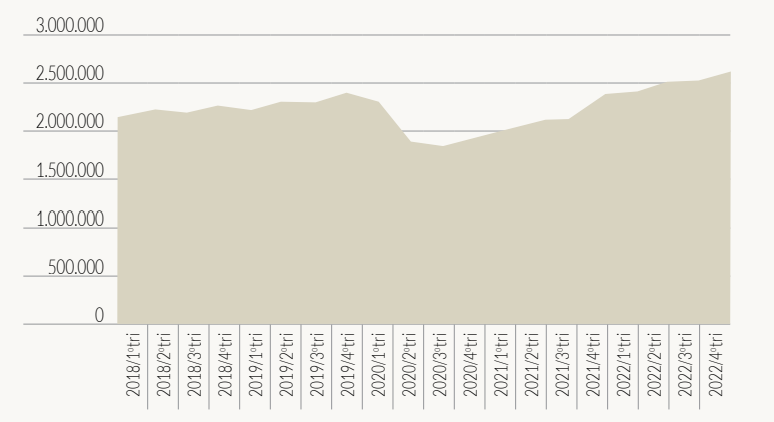
\includegraphics[width=0.9\textwidth]{cap01-Introducao/Images/1.3_grafico_profissionais_brasil}
 	\label{fig:profissionais_brasil}
 	\fonte{\cite{senac_panorama_mercado}}
 \end{figure}
 
 \FloatBarrier
 
Dentre o constante crescimento de profissionais neste setor, os cabeleireiros representam a maioria, conforme indica o gráfico abaixo (\ref{fig:Distribuição_profissionais}).

%inicio de figura
\begin{figure}[htb]
	\centering
	\caption{Distribuição dos profissionais da área da beleza 2018-2021}
	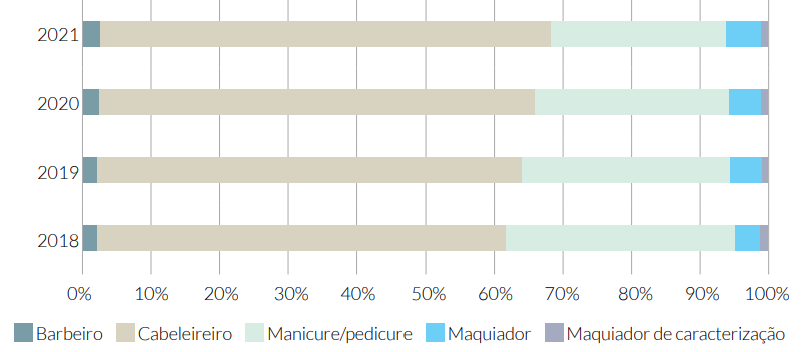
\includegraphics[width=0.9\textwidth]{cap01-Introducao/Images/1.3_grafico_maioria_cabeleireiros}
	\label{fig:Distribuição_profissionais}
	 \fonte{\cite{senac_panorama_mercado}}
\end{figure}

\FloatBarrier

Apesar da expressividade econômica, o setor enfrenta desafios operacionais que limitam a rentabilidade e a eficiência dos empreendedores. Dados indicam que: 

\begin{itemize}
	\item Até 30\% do tempo de um pequeno empreendedor é consumido por tarefas administrativas \cite{senac2022};
	\item Taxa média de não comparecimento de clientes atinge 25\% \cite{booksy2022};
	\item Perda de 20\% da receita por não comparecimento \cite{abihpec2021};
	\item Média de 15 horas semanais são dedicadas ao controle manual de agenda e finanças \cite{fgv2020};
	\item Insatisfação de 40\% dos clientes devido a falhas de comunicação e alterações de última hora \cite{mindminers2022}.
\end{itemize}

Como resposta à necessidade de reduzir custos fixos e aumentar a flexibilidade, o modelo de \emph{coworking}, originado em ambientes de escritório, expandiu-se para o setor da beleza, permitindo o compartilhamento de espaços e recursos e a redução de custos \cite{sebrae_coworking,sebraesc2025}. Anteriormente à popularização dos \emph{cowrokings} de beleza, os profissionais se distribuiam em diversos locais para economizar recursos, como mostra a figura \ref{fig:Distribuição_locais}:

%inicio de figura
\begin{figure}[htb]
	\centering
	\caption{Distribuição dos profissionais da área da beleza por local de trabalho 2018-2022}
	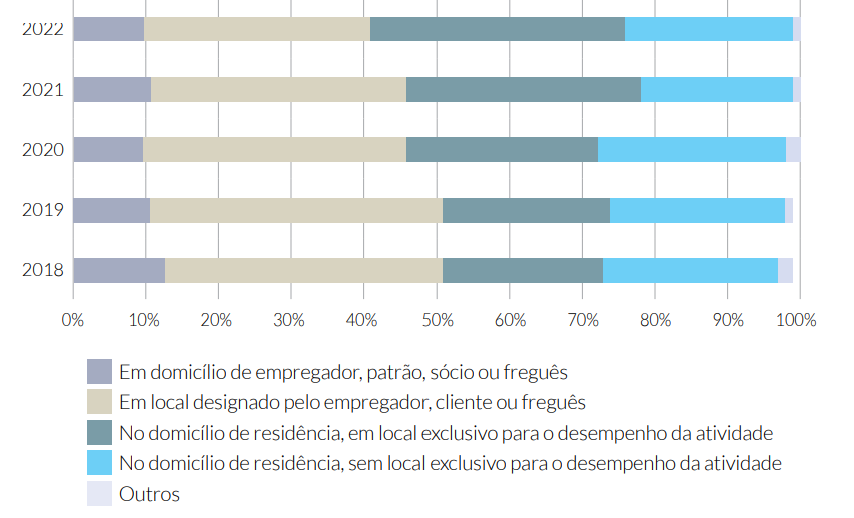
\includegraphics[width=0.9\textwidth]{cap01-Introducao/Images/1.3_local_trabalho_profissionais}
	\label{fig:Distribuição_locais}
	\fonte{\cite{senac_panorama_mercado}}
\end{figure}

\FloatBarrier

Embora solucione a questão do investimento em infraestrutura, esse modelo introduz novas complexidades relacionadas à gestão compartilhada de espaços, agendamentos e finanças. Portanto, nesse contexto justifica-se o projeto de extensão \emph{BS Beauty}, uma aplicação \emph{web} customizada para o gerenciamento de salões em modelo \emph{coworking}, sob a coordenação de nossa parceira de extensão Bruna. Ao digitalizar e centralizar processos principais, a BS Beauty empodera pequenos empreendedores por meio da redução de custos operacionais e erros humanos. O sistema oferece controle preciso de comissões e frequências, ao passo que \emph{dashboards} e relatórios financeiros detalhados fornecem \emph{insights} estratégicos para o negócio. 

Dessa forma, a plataforma não apenas soluciona os desafios de gestão administrativa, mas também aprimora a experiência do cliente e gera valor para todos os envolvidos. Além disso, como iniciativa de extensão, o projeto simultaneamente permite que os alunos‐desenvolvedores apliquem e aprimorem conhecimentos técnicos e de gestão, enfrentando desafios reais de mercado e aproximando a graduação da prática profissional.


